\newcommand{\program}{Finančna matematika}
\newcommand{\imeavtorja}{Nejc Duščak}
\newcommand{\imementorja}{izr. prof. dr. Janez Bernik}
\newcommand{\naslovdela}{Realne opcije}
\newcommand{\letnica}{2021}
\newcommand{\povzetek}{V diplomski nalogi sem želel pokazati glavne razlike med tradicionalnimi in realnimi metodami za vrednotenje različnih investicij. S primeri sem poskušal še bolj ponazoriti glavne razlike. Glavni problem je bilo vrednotenje managerske fleksibilnosti, ki lahko močno spremeni vrednost investicije. S različnimi vrstami realnih opcij (opcija časa investiranja, opcija rasti, opcija zožitve in opcija opustitve projekta) sem pokazal kako pravilno in najbolje vrednotiti fleksibilnost in kako to vpliva na vrednost celotne investicije. Te metode so se izkazale kot zelo primerne za vrednotenje investicij, saj zajemajo veliko spremenljivk, ki lahko močno zanihajo vrednost investicije. Zato menim, da so metode zelo uporabne, vendar je sama investicija še veliko bolj kompleksna in je na področju vrednotenja še veliko spremenljivk, ki jih je težko in jih še ne znamo vrednotiti.}
\newcommand{\kljucnebesede}{realne opcije\sep tradicionalne metode vrednotenja\sep finančne opcije\sep uporaba realnih opcij}

% Če ne deluje, zakomentiraj naslednjo vrstico in odkomentiraj naslednji dve
\begin{filecontents*}[overwrite]{\jobname.xmpdata}
% \RequirePackage{filecontents}
% \begin{filecontents*}{\jobname.xmpdata}
\Title{\naslovdela}
\Author{\imeavtorja}
\Language{sl-SI}
\Subject{\povzetek}
\Keywords{realne opcije\sep tradicionalne metode vrednotenja\sep finančne opcije\sep uporaba realnih opcij}
\end{filecontents*}
\documentclass[12pt, a4paper]{amsart}
\usepackage[a-1b]{pdfx} 
\usepackage{array}
\newcolumntype{L}{>{\centering\arraybackslash}m{6,5cm}}
\usepackage[utf8]{inputenc}
\usepackage[T1]{fontenc}
\usepackage[slovene]{babel}
\usepackage{colorprofiles}
\hypersetup{pdfstartview=}
\usepackage{lmodern}
\usepackage{amsmath}
\usepackage{units}
\usepackage{eurosym}
\usepackage{amsfonts}
\usepackage{fancyhdr,amssymb,amsmath,amsthm,bbm,enumerate,mdwlist,url,multirow,hyperref,graphicx}
\usepackage{pdfpages}
\usepackage{comment}
\usepackage{breqn}
\usepackage{caption}
\usepackage{subcaption}
\usepackage{float}
\usepackage{graphicx}
\usepackage{amssymb}
\usepackage{tikz}
\usepackage{nicefrac,xfrac}
\usepackage{enumerate}
\setlength{\parindent}{0mm}

% ne spreminjaj podatkov, ki vplivajo na obliko strani
\textwidth 15cm
\textheight 24cm
\oddsidemargin.5cm
\evensidemargin.5cm
\topmargin-5mm
\addtolength{\footskip}{10pt}
\pagestyle{plain}
\overfullrule=15pt % oznaci predlogo vrstico


% ukazi za matematicna okolja
\theoremstyle{definition} % tekst napisan pokoncno
\newtheorem{definicija}{Definicija}[section]
\newtheorem{primer}[definicija]{Primer}
\newtheorem{opomba}[definicija]{Opomba}

\renewcommand\endprimer{\hfill$\diamondsuit$}


\theoremstyle{plain} % tekst napisan posevno
\newtheorem{lema}[definicija]{Lema}
\newtheorem{izrek}[definicija]{Izrek}
\newtheorem{trditev}[definicija]{Trditev}
\newtheorem{posledica}[definicija]{Posledica}

\def\sep{, }

% za stevilske mnozice uporabi naslednje simbole
\newcommand{\R}{\mathbb R}
\newcommand{\N}{\mathbb N}
\newcommand{\Z}{\mathbb Z}
\newcommand{\Q}{\mathbb Q}

\providecommand{\C}{}
\renewcommand{\C}{\mathbb C}

% ukaz za slovarsko geslo
\newlength{\odstavek}
\setlength{\odstavek}{\parindent}
\newcommand{\geslo}[2]{\noindent\textbf{#1}\hspace*{3mm}\hangindent=\parindent\hangafter=1 #2}

\begin{document} 
\raggedbottom
\thispagestyle{empty}
\noindent{\large
UNIVERZA V LJUBLJANI\\[1mm]
FAKULTETA ZA MATEMATIKO IN FIZIKO\\[5mm]
Finančna matematika -- 1.~stopnja}
\vfill

\begin{center}{\large
\imeavtorja\\[2mm]
{\bf \naslovdela}\\[10mm]
Delo diplomskega seminarja\\[1cm]
Mentor: \imementorja}
\end{center}
\vfill

\noindent{\large
Ljubljana, \letnica}
\pagebreak

\thispagestyle{empty}
\tableofcontents
\listoffigures
\listoftables
\pagebreak

\thispagestyle{empty}
\begin{center}
{\bf \naslovdela}\\[3mm]
{\sc Povzetek}
\end{center}
\povzetek
\vfill
\begin{center}
{\bf Real options}\\[3mm] 
{\sc Abstract}
\end{center}
In my thesis I aimed to show  main differences between the traditional and real valuation methods of various investments. I aimed to show differences through cases and examples. Main problem was within the value of managarial flexibility which can considerably change the value of investment. Through various examples of real options (option to defer investment, option to expand, option to contract, option to abandon) I displayed how to correctly and effectively valuate flexibility. Morever, I showed how such flexibility affects the overall valuation. Those methods proved to be sufficiently appropriate for the valuation of investments as they encompass wide spectrum of variables which can influence the value of investment. Thus, in my opinion those methods proved to be valuable as well as useful, although there are further complexities in an investment, some even  beyond our understanding.

\vfill\noindent
{\bf Math. Subj. Class. (2010):} 	91-00   \\[1mm]  
{\bf Klju"cne besede:} \kljucnebesede  \\[1mm]
{\bf Keywords:} real options, traditional valuation methods, financial options, real options in practice
\pagebreak


\section{Uvod}
Odločitev za investiranje v projekt je eden izmed osnovnih problemov, s katerim se srečujejo podjetja. Ne glede na velikost podjetja, je problem investiranja ključen za možnost uspešnega nadaljnjega razvoja. Pri izbiri različnih investicij so se skozi zgodovino oblikovali številni modeli za vrednotenje investicij, saj podjetja le na podlagi svojih občutkov in ugibanj težko sprejemajo odločitve, ki se bodo izkazale kot uspešne. Zato je za podjetja pomembno, da se odloča za dobre in predvsem uspešne metode vrednotenja in s tem poveča možnost dobre naložbe, kar bi povečalo vrednost podjetja in posledično tudi premoženje delničarjev. Prav tako pa management z uporabo investicijskih metod predstavi investicijo in na eni strani prepriča vlagatelje, na drugi strani pa delničarjem utemelji smiselnost investicije.\\

Poznamo številne metode vrednotenja investicije, kot so metoda neto sedanje vrednosti (NSV), notranja stopnja donosa (IRR), popravljena stopnja donosa, ekonomski dobiček, drevo odločanja in ostale. V praksi je največkrat uporabljena metoda neto sedanje vrednosti, saj je njena uporaba preprosta in dokaj zanesljiva. Več o tej metodi bomo povedali v nadaljevanju diplomske naloge. \\

Pri investiciji pa je tudi zelo pomembno razumeti tveganje. Zaradi neprestanega spreminjanja tržnih razmer, povpraševanje po dobrinah in hitro rastoča tehnologija so faktorji, ki vplivajo na tveganje. Zato si je potrebno vzeti dovolj časa, da pravilno ocenimo tveganje in s tem zagotovimo najboljše vrednotenje investicij. Na samo investicijo pa vplivajo tudi regulativne omejitve. To so omejitve, ki omejujejo sposobnost podjetja, da maksimizira svoje cilje, ki jih ponavadi opišemo s ciljno funkcijo. Šele ko dobro razumemo vse te dejavnike, lahko oblikujemo metodo realnih opcij, saj ta metoda omogoča razumevanje vpliva stroškov regulativnih omejitev na celotne stroške, ki nastanejo zaradi zamud in podobnih problemov. V zadnjih letih pa je uporaba metode realnih opcij narasla, saj upošteva tudi fleksibilnost managementa, ki ob neugodnih razmerah investicijo prekine ali zmanjša proizvodnjo, ob ugodnih razmerah pa investicijo razširi. Zato menim, da je kljub dejstvu, da je za metodo realnih opcij potrebno več znanja in denarja (zaradi dodatnih raziskav trga in podjetja), ta metoda uporabna in nujna za kvalitetno oceno investicije.   \\   

Namen diplomske naloge je predstavitev metode realnih opcij kot še ene izmed metod vrednotenja investicij, ki se je izkazala kot dobra alternativa tradicionalnim metodam in izboljšala sprejemanje investicij. \\

\pagebreak

\section {Tveganje in investicije}
Investicijske odločitve lahko opredelimo kot najpomembnejše odločitve v podjetju. Podjetje z investicijami zagotavlja rast in dolgoročno preživetje, prav tako pa ohranja konkurenčni položaj na trgu in  sledi razvoju konkurenčnih podjetij. Zato mora podjetje investicijskemu oziroma finančnemu načrtovanju dolgoročnih naložb posvečati veliko pozornosti. Pomembno je, da podjetje sledi cilju poslovanja, pri katerem želi predvsem maksimizirati vrednost podjetja. Vsako investicijo pa sestavljajo trije ključni postopki:
\begin{enumerate}
\item{Načrtovanje investicije}: v tem delu investicije podjetje identificira problem. V podjetju začnejo z iskanjem rešitev, ki privedejo do investicijskih predlogov. Te predloge finančno vrednotijo (presodijo upravičenost investicije) in jih na podlagi metod sprejmejo ter zagotovijo vire financiranja.
\item{Izvedba investicijskega projekta}: v podjetju se začnejo odvijati dejavnosti, ki so neposredno povezane z investicijo, kot so na primer investicijski izdatki, prva proizvodnja in prodaja.
\item{Nadzor in ukrepanje}: gre za nadzor nad izdatki in ustvarjenim donosom.
\end{enumerate}

V samem investicijskem odločanju pa je prisotno tudi investicijsko tveganje, ki lahko spremeni potek investicije in v najslabšem primeru pripelje do propada podjetja. Zato bi se rad v nadaljevanju razdelka posvetil tveganju.\\

Za začetek se vprašajmo, kaj je tveganje in zakaj se o njem pogovarjamo?\\
Tveganje opredelimo kot verjetnost, da se bo zaradi zunanjih ali notranjih vplivov zgodila škoda. Tveganje je možnost, da bo končni izid drugačen od pričakovanega, oziroma nam preprečuje doseganje ciljev. V primeru investicij je tveganje možnost, da bo dejanski donos različen od pričakovanega. Naš namen je razumeti obnašanje investitorjev in ugotoviti kako ocenjujejo tveganje investicije. Na podlagi tveganja pa se tudi določi zahtevana stopnja donosa. Zato je za management pomembno kako se ga meri, saj to omogoča, da se izognejo nepotrebnim izgubam \cite{investopedia}. \\

Vsak posameznik je vsako dnevno izpostavljen tveganju. Prav tako pa je vsak posameznik različno naklonjen tveganju, zato rečemo, da ima vsak investitor svoj profil tveganja. Nekateri so tveganju bolj naklonjeni, zato bodo sprejemali investicije z višjim tveganjem, medtem ko jih bodo drugi zavrnili že pri veliko manjšem tveganju. V splošnem pa lahko rečemo, da so investitorji tveganju nenaklonjeni, kar pomeni, da če gledamo investicije v katerih se spreminja samo tveganje, jim manj tvegane prinašajo višjo koristnost. To pomeni, da bodo v primeru enakih koristnosti izbrali investicijo z manjšim tveganjem, v primeru enakega tveganja, pa bodo izbrali investicijo z višjo koristnostjo \cite{Crnigoj}. \\

Pri tveganju je pomembno omeniti tudi povezavo s časovnim horizontom. Ta je pogosto glavni dejavnik, ki vpliva na ocenjevanje tveganja. Če bo investitor želel, da je njegov vložek povrnjen v najkrajšem možnem času, bo nenaklonjen investiranju v projekt, ki mu ne zagotavlja hitrih donosov, vendar bo svoj denar raje vložil v manj tvegane projekte. Prav tako bodo mlajši investitorji bolj naklonjeni investiranju v bolj tvegane projekte, ki imajo višje donose \cite{investopedia}. \\

Realne opcije pa niso uporabne samo v primeru ocene investicije, ampak so uporabno orodje tudi v primeru kapitalskih investicij. Na primer, ali naj podjetje investira nekaj milijonov v najnovejšo tehnologijo? Kako naj podjetje izbere med številnimi ponudbami? Ali naj podjetje vloži denar tudi v raziskave trga? V tradicionalnih modelih diskontiranih denarnih tokov, ne moremo z gotovostjo odgovoriti na takšna vprašanja. Še več, nekateri odgovori, so lahko povsem napačni.  Model realnih opcij pa upošteva oblikovanje projekta pod vplivom tveganja in managementa, ki lahko v vsakem trenutku spremeni potek investicije. \\


\section{Tradicionalne metode vrednotenja investicij}
V tem razdelku bom opisal tradicionalne metode vrednotenja imenovane tudi modeli diskontiranih denarnih tokov. Osredotočil se bom na opis nekaterih metod in prikazal pomanjkljivosti teh modelov, zaradi katerih se uporaba realnih opcij zdi veliko bolj primerna. Tu predvsem mislim na dejstvo, da tradicionalni modeli ne upoštevajo vpliv fleksibilnosti.

Pri uporabi tradicionalnih modelov vrednotenja je vrednost definirana kot diskontirana časovna vrednost, ki predstavlja denarne tokove v prihodnosti. V nasprotju s to definicijo, je dejstvo, da so sredstva na trgu prodana za ceno, ki ni nujno enaka realni vrednosti. Zato je ideja vrednotenja, oblikovanje poštenega trga, kjer je cilj določiti vrednost sredstva zelo blizu njegove realne vrednosti. V preteklosti so se oblikovali trije glavni pristopi vrednotenja sredstev, imenovani tržni pristop \textit{(angl. the market approach)}, dohodkovni pristop \textit{(angl. the income approach)} in stroškovni pristop \textit{(angl. the cost approach)} \cite[str. 63]{Mun}.\\

\textbf{Tržni pristop} upošteva cene primerljivih sredstev na trgu in predpostavlja, da bo tržna moč oblikovala ravnotežno ceno. Predpostavlja tudi, da je tržna cena pravična cena, ko ji odštejemo stroške poslovanja in vpliv tveganja. \\

\textbf{Dohodkovni pristop} je pristop, ki pogleda dosegljivo prihodnjo vrednost sredstva in jo poskuša izmeriti, napovedati in diskontirati na sedanjo vrednost. Ko od dobljene vrednosti odštejemo stroške izvedbe, nakupa in razvijanja sredstva, dobimo neto sedanjo vrednost. Za diskontno stopnjo pa uporabimo tehtano povprečje stroškov kapitala (\textit{angl. WACC}).\\

\textbf{Stroškovni pristop} obravnava stroške, ki bi jih imelo podjetje, če bi zamenjalo ali reproduciralo dosegljivo prihodnjo vrednost sredstva, kjer upoštevamo tudi neopredmetene stroške.\\

Obstajajo pa tudi številni drugi pristopi, ki se osredotočajo na vrednotenje neopredmetenih sredstev, s tem mislim na oceno imena podjetja ali pa njegove blagovne znamke. Na primer podjetje Nike lahko za svoje izdelke postavi višjo ceno, zaradi svoje prepoznavnosti. Pri tem vrednotenju se vrednost določi glede na to, kaj sredstvo prinese glede na ekonomski pomen \cite[str. 64, 65]{Mun}. \\

\subsection{Praktični problemi uporabe tradicionalnih metod}
Pri uporabi tradicionalnih metod vrednotenja, ki za svoje izračune uporabljajo diskontirane denarne tokove, se lahko pojavijo napake pri oceni investicijskih priložnosti. Tradicionalne metode predpostavijo, da se investicija zgodi v celoti ali pa se ne zgodi. Ne upoštevajo fleksibilnosti managementa, ki lahko spremeni potek investicije, ko negotovost postaja vse bolj jasna. In prav to je ena izmed glavih razlik v primerjavi z realnimi opcijami, pri katerih se dopušča možnost upravljanja z investicijo tudi po zagonu le-te \cite[str. 65, 66]{Mun}.\\
Kljub številnim slabim lastnostim uporabe teh modelov, pa imajo ti modeli tudi nekaj prednosti \cite[str. 66]{Mun}:
\begin{itemize}
\item jasen, konstanten odločitveni kriteriji za vsak projekt,
\item enaki rezultati ne glede na preference tveganja investitorjev,
\item zadosten nivo natančnosti in ekonomske racionalnosti,
\item relativno enostaven in hitro učljiv,
\item enostaven za utemeljitev smiselnosti investicije.
\end{itemize}
V realnosti se mora investitor zavedati pomanjkljivosti metod diskontiranih denarnih tokov. Hitro lahko pride do podcenjevanja sredstev, ki na začetku prinašajo nizke donose ali pa v najslabšem primeru prinašajo ničelne donose. Prav tako pri diskontiranju denarnih tokov uporabljamo konstanten faktor tehtanega povprečja stroškov kapitala (WACC), ki pa je v resnici nekonstanten. Tudi ocenjevanje prihodnjih denarnih tokov ni nujno pravilno. Največji problem pa so dejstva poslovne realnosti. S tem mislim tveganje, pravi čas za izvedbo investicije in fleksibilnost managementa. V današnjem svetu lahko uporaba diskontiranih denarnih tokov močno zamegli pravo vrednost investicije, saj predpostavlja poslovni svet, v katerem so vsi prihodnji denarni tokovi fiksni in svet v katerem ne prihaja do nikakršnih nihanj, ki bi lahko spremenili vrednost projekta. Tako rekoč fleksibilnost ne bi imela nikakršne vrednosti. Vemo pa, da če bi imel management možnost fleksibilnosti, ki bi povečal vrednost projekta, bi to tudi storil, zato je uporaba fleksibilnosti nujna pri vrednotenju investicij \cite[str. 66]{Mun}.\\

\pagebreak
\begin{table}[ht]
	\caption{Predpostavke tradicionalnih modelov in realnost}
	\centering
	\begin{tabular}{|L|L|}
	\hline
	\textbf{Predpostavke tradicionalnih modelov} & \textbf{Realnost} \\
	\hline
	\hline
	Odločitve so sprejete v trenutku, zato so denarni tokovi v prihodnosti fiksni. & Zaradi negotovosti in tveganja so prihodnji denarni tokovi težko napovedljivi. Odločitve niso nujno sprejete v trenutku, ampak jih lahko sprejmemo tudi kasneje, ko del negotovosti postane jasen. \\
	\hline
	Investicijo gledamo kot mini podjetje. &  Investicija vpliva na različna področja v podjetju, zato težko ocenimo njen vpliv. \\
	\hline
	Ko investicijo zaženemo, jo pustimo pri miru. & Investicija se spremlja skozi celoten življenjski cikel, saj se lahko med njo stvari spremenijo. \\
	\hline
	Prihodnji denarni tokovi so napovedljivi in točni. & V realnosti je zaradi tveganja težko pravilno napovedati denarne tokove. \\
	\hline
	Diskontna stopnja je enaka oportunitetnemu strošku kapitala. & Obstajajo številni različni vplivi na diskontno stopnjo, ki se lahko skozi investicijo tudi spreminjajo.\\
	\hline
	Diskontna stopnja upošteva vsa tveganja, ki so prisotna. & Tveganja se skozi čas spreminjajo, zato težko določimo pravilno diskontno stopnjo. \\
	\hline
	Vsi faktorji, ki bi lahko vplivali na prihodek investicije, so upoštevani v denarnem toku. & Težko je napovedati in upoštevati vse denarne tokove, ki bodo nastali kot posledica investicije. \\
	\hline
	Nepoznani, neopredmeteni in nemerljivi faktorji so enaki 0. & Neopredmetena sredstva predstavljajo pomemben del sredstev. \\
	\hline
	\end{tabular}
\end{table} 
(Vir: \cite[str. 67]{Mun})



Pri uporabi tradicionalnih metod vrednotenja je najbolj občutljiva spremenljivka diskontna stopnja. Ponavadi se v teh primerih uporablja tehtano povprečje stroškov kapitala, ki je s pogleda managementa nujno za vsako podjetje. Prav tako je diskontna stopnja spremenljivka, ki jo je najtežje pravilno napovedati oziroma bolje rečeno oceniti. Zato dopušča manipuliranje in prilagajanje rezultatov. Na primer, želena NSV je lahko dosežena z zelo malim odmikom diskontne stopnje. Na drugi strani pa so tudi metode za določitev diskontne stopnje lahko vprašljive. Metoda WACC, kjer je strošek lastniškega kapitala običajno določen z uporabo modela CAMP, v katerem pa nastopa tako imenovani beta koeficient (tržno tveganje), ki ga je prav tako težko oceniti. Beta koeficient je občutljiv faktor, ki meri povezave med ceno lastniškega kapitala in upoštevanjem trga. Problem je, ker se lastniški kapital spreminja vsakih par minut. Zato je izračun beta koeficient za finančna sredstva lahko nevaren \cite[str. 69, 70]{Mun}.\\
 
V nadaljevanju  bom opisal nekatere tradicionalne modele vrednotenja, katere bom ponazoril s primeri uporabe za lažjo predstavo.

\subsection{Metoda neto sedanje vrednosti}
Metoda neto sedanje vrednosti (angl. net present value) nam pove, ali je investicija upravičena ali ne. Pri njenem izračunu uporabljamo načelo sedanje vrednosti. Tako na eni strani izračunamo sedanjo vrednost naložbe, na drugi strani pa sedanjo vrednost vseh izdatkov, ki so in bodo pri investiciji nastali. Njuna razlika se imenuje neto sedanja vrednost. Če poenostavim, nam neto sedanja vrednost pove, ali smo za osnovna sredstva, oglaševanje, znanje itd., plačali več (ali manj) kot pa je njihova vrednost za podjetje. V realnosti le malokdaj uporabimo tako strogo predpostavko. Neto sedanjo vrednost izračunamo z spodnjo formulo: \\

\begin{center}
$  NSV = \tfrac{DT_1}{1+r} + \tfrac{DT_2}{(1+r)^2} + ... + \tfrac{DT_n}{(1+r)^n} - I_0 $ \\,
\end{center}

kjer $DT_n$ označuje denarni tok, ki bo nastal v času $n$, $I_0$ izdatek ob času 0 in $r$ zahtevano stopnjo donosa \cite[str. 154]{Mramor}. \\

Vsi denarni tokovi, ki se bodo pri investiciji pojavili v prihodnosti, so v enačbi diskontirani z ustrezno diskontno stopnjo na čas 0. To omogoča, da izvemo, kakšna je vrednost investicije danes in se tako lahko najbolje  odločimo. V primeru, da je izračunana NSV negativna, bomo investicijo zavrnili, v nasprotnem primeru jo bomo sprejeli. Na kratko to lahko zapišemo kot:

\begin{itemize}
\item $NSV \geq 0$: investicijo sprejmemo,
\item $NSV<0$: investicijo zavrnemo.
\end{itemize}

\subsubsection{Primer: Kako izračunati NSV?}
Podjetje Korenček presoja o nakupu nove strojne opreme. Oprema stane $100$ €, njihova notranja stopnja donosa pa znaša $10$ \%. Investicijski donosi so podani v spodnji preglednici. Izračunaj NSV. \\

\begin{table}[ht]
	\caption{Denarni tokovi za izračun NSV}
	\centering
	\begin{tabular}{|L|L|}
	\hline
	\textbf{Leto} & \textbf{Denarni tok} \\
	\hline
	\hline
	0&-100\\
	\hline
	1&10\\
	\hline
	2&60\\
	\hline
	3&80\\
	\hline
	\end{tabular}
\end{table}

Izračun NSV:\\
$NSV = -100 + \tfrac{10}{1+0,1} + \tfrac{60}{(1+0,1)^2} + \tfrac{80}{(1+0,1)^3}$ \\[0,5 cm]
$NSV = 18,78$ €  \\

Ker je vrednost pozitivna, bomo investicijo sprejeli.

\subsection{Interna stopnja donosa}
Interna stopnja donosa \textit{(angl. internal rate of return)} je metoda, ki je v praksi lažje razumljiva kot metoda neto sedanje vrednosti. Kot rezultat izračuna dobimo, kolikšna je (notranja) donosnost investicije. Pravzaprav dobimo diskontno stopnjo, ki enači prihodnje denarne tokove s prvotnimi izdatki za investicijo. Zato lahko ugotovimo, da izračun temelji na uporabi neto sedanje vrednosti. Pri izračunu si pomagamo s spodnjo formulo \cite[str. 156]{Mramor}:\\

\begin{center}
$I_0 = \tfrac{DT_1}{1+k} + \tfrac{DT_2}{(1+k)^2} + ... + \tfrac{DT_n}{(1+k)^n}$,\\
\end{center}

kjer je $DT_n$ denarni tok v času n, $k$ notranja stopnja donosa in $I_0$ začetni izdatki. \\

Kriterij za sprejem odločitve pri uporabi te metode je naslednji: investicijo sprejmemo, če je interna stopnja donosa večja ali enaka zahtevani stopnji donosa, za katero največkrat uporabimo kar tehtano povprečje stroškov kapitala (angl. WACC) ali pa vzamemo zahtevano stopnjo donosa sorodnih investicij. V primeru, ko je notranja stopnja donosa manjša od zahtevane stopnje, pa investicijo zavrnemo. Če poenostavimo:

\begin{itemize}
\item IRR $\geq$ zahtevana stopnja donosa: investicijo sprejmemo,
\item IRR $<$ zahtevana stopnja donosa: investicijo zavrnemo.
\end{itemize}


Kljub vsem svojim prednostim je lahko izračun notranje stopnje donosa težaven. Izračun se močno poenostavi, ko denarni tokovi nastopajo zgolj v začetnem in končnem obdobju, se pravi v dveh obdobjih. Na primer, začetni izdatki za investicijo znašajo $100$ €, denarni tok na koncu obdobja pa $120$ €. Predpostavimo, da gre zgolj za eno obdobje. Potem rešitev dobimo kot \cite[str. 157]{Mramor}:\\

\begin{center}
$100 = \tfrac{120}{1+k}$\\[0,5cm]
$k = \tfrac{120}{100} - 1$\\[0,5 cm]
$k = 0,2$
\end{center}

Težava nastopi, ko se denarni tokovi pojavijo v več kot dveh obdobjih. Takrat izračun interne stopnje donosa analitično ni možen. V tem primeru si pomagamo z metodo poskusov in napak. Pri tej metodi gre za to, da se s poskusi vstavljanja različnih stopenj donosa želimo čim bolj približati vrednosti na levi strani enačbe oziroma začetnim izdatkom. Da bo bolje razumljivo, bom to metodo ponazoril na primeru. Predpostavimo, da je donos naložbe konec prvega leta znašal $10$ €, konec drugega pa $60$ €. Naložba je na začetku zahtevala $50$ € izdatkov. Sedaj pa želimo poiskati stopnjo donosa s pomočjo naslednje enačbe \cite[str. 158]{Mramor}:\\

\begin{center}
$50 = \tfrac{10}{1+r} + \tfrac{60}{(1+r)^2}$,
\end{center}
kjer $r$ predstavlja stopnjo donosa, ki jo želimo najbolje oceniti z metodo poskusov in napak.

\begin{table}[ht]
\caption{Primer uporabe metode poskusov in napak za izračun IRR}
\begin{tabular}{|c|c|c|c|}
\hline
Stopnja donosa & \begin{tabular}[c]{@{}c@{}}Sedanja vrednost donosov\\naložbe\end{tabular} & \begin{tabular}[c]{@{}c@{}}Sedanja vrednost\\izdatkov naložbe\end{tabular} & Razlika \\ \hline
\hline
0,15           & 54,1                                                                       & 50                                                                          & 4,1     \\ \hline
0,25           & 46,4                                                                       & 50                                                                          & -3,6    \\ \hline
0,2            & 50                                                                         & 50                                                                          & 0       \\ \hline
\end{tabular}
\end{table}
(Vir: \cite[str. 158]{Mramor})\\

Tako smo videli, da sta pri stopnji donosa $0,2$ leva in desna stran enačbi enaki, kar pomeni, da smo našli rešitev. \\

\subsection{Doba povračila}
Ta metoda nam kot rezultat ponudi število let, v katerih se nam bo vloženi znesek povrnil. Če je doba povračila dovolj kratka, da je z njo zadovoljen manager, potem bo seveda investicijo podprl, v nasprotnem primeru pa jo bo zavrnil. Seveda je zaželeno, da je doba povračila čim krajša. Zato tudi v primeru dveh izključujočih investicij, izberemo tisto s krajšo dobo. Pri sami metodi je pomembno, da poleg neto donosov upoštevamo tudi amortizacijo, saj tako dobimo boljši rezultat \cite[str.153]{Groppelli}.\\

\subsubsection{Uporaba dobe povračila za oceno investicije}
ABC podjetje namerava investirati v projekt z začetnimi izdatki v višini $3700$ €. Napovedano je, da bo projekt prinašal naslednje donose: $1000$ € v prvem letu, $2000$ € v drugem letu, $1500$ € v tretjem letu in $1000$ € v četrtem letu. Kakšna je doba povračila?\\
Vidimo lahko, da bo imelo podjetje po dveh letih pokrito $3000$ € svoje investicije. Da bi pokrili celotno začetno investicijo jim primanjkuje še $700$ €. Doba povračila je tako enaka \cite[str. 154]{Groppelli}:

\begin{center}
$2 + \tfrac{700}{1500} = 2 + 0,47$
\end{center}
Dobimo rezultat $2$ leti in $24$ mesecev.\\


\section{Finančne opcije}
Za začetek bi rad opisal finančne opcije in njihove značilnosti, saj bomo le tako kasneje razumeli delovanje in pomanjkljivosti realnih opcij.\\

Finančna opcija je instrument oziroma pogodba pri kateri ima kupec opcije možnost, da se odloči ali bo opcijo izvršil ali ne. Finančna opcija se nanaša na osnovno premoženje, kjer je možen nakup ali prodaja le-tega po določeni ceni $K$, ki jo imenujemo izvršilna cena. Nosilca opcije imenujemo tudi dolga stran \textit{(angl. option holder)}, izdajatelja pa kratka stran \textit{(angl. option writer)}. Če ima nosilec opcije možnost nakupa osnovnega premoženja, opcijo imenujemo nakupna opcija \textit{(angl. call option)}, če pa daje pravico prodaje, jo imenujemo prodajna opcija \textit{(angl. put option)}. Glede na to kdaj bomo opcijo izvršili ločimo več vrst opcij \cite[str. 53, 54 ]{Kosir}:
\begin{itemize}
\item evropska opcija daje pravico izvršiti opcijo le ob zapadlosti,
\item ameriška opcija daje pravico izvršiti opcijo kadarkoli do vključno trenutka zapadlosti,
\item eksotične opcije pa so opcije, ki imajo svoja pravila.
\end{itemize}
Tako lahko opazimo glavno prednost finančnih opcij, ki daje nosilcu pravico ne pa obveznosti. Vedeti moramo tudi, da nosilec opcije ob nakupu opcije plača premijo za opcijo \textit{(angl. option premium)} in potem nima več obveznosti, ampak le še pravice. Izdajatelj opcije pa mora pri klirinški hiši voditi vzdrževalni račun, s katerim dokazuje, da je zmožen izpeljati dogovorjen posel \cite[str. 54]{Kosir}.\\

Sedaj si poglejmo, kako analiziramo vrednost evropske in ameriške nakupne ter prodajne opcije. S $t=0$ označimo čas, ko je opcija izdana, s $t=T$ pa označimo čas zapadlosti. $S_t$ je vrednost osnovnega premoženja ob času $t$. S $K$ pa označimo izvršilno ceno. Nosilec opcije bo opcijo izvršil, če bo razlika med ceno osnovnega premoženja in izvršilno ceno zanj pozitivna. V nasprotnem primeru opcije ne izvrši in je njena vrednost enaka $0$. S $C_t$ označimo vrednost nakupne opcije in $P_t$ vrednost prodajne opcije ob času $t$. Ker vemo, da je nosilec opcije racionalen in želi zase le najbolje, bo nakupno opcijo izvršil, če je $S_t > K$, prodajno pa bo izvršil, če je $S_t < K$ \cite[str. 54-58]{Kosir}.\\

Tako dobimo izplačilo evropske opcije ob času $T$ kot:
\begin{center}
$C_T = max\{S_T - K; 0\}$\\
$P_T = max\{0; K - S_T\}$
\end{center}  
Zgornji formuli sta enaki tudi za ameriško opcijo v primeru, ko je ne izvršimo pred zapadlostjo. Drugače pa vrednost ameriške opcije izračunamo po formuli:\\
Tako dobimo izplačilo ameriške opcije ob času $t$ kot:
\begin{center}
$C_t = max\{S_t - K; 0\}$\\
$P_t = max\{0; K - S_t\}$
\end{center}  
Če je $C_t>0 (P_t>0)$, rečemo, da se opcija splača, če je $S_t=K$ rečemo, da je opcija na meji, v primeru, ko je $C_t<0 (P_t<0)$, pa rečemo, da se opcija ne splača.\\
Za osnovno razumevanje opcij je zgornja razlaga popolnoma dovolj. Če bi želeli, bi lahko razložili tudi različne strategije trgovanja z opcijami in vpliv premij na samo vrednost opcije \cite[str. 54-58]{Kosir}.

\subsection{Realne in finančne opcije}
V tem poglavju bom govoril o razlikah med realnimi in finančnimi opcijami, in o razumevanju, da teorija realnih opcij stoji na teoriji finančnih opcij, vendar je kljub temu med njima veliko razlik. Te razlike je pomembno razumeti, saj vplivajo na oblikovanje in uporabo matematičnega modela realnih opcij. \\

Realne opcije dopolnjujejo finančne opcije v smislu analize realnih in fizičnih stvari. Med njima je tudi nekaj podobnosti, vendar se bom bolj osredotočil na razlike, ki so nazorno prikazane tudi v tabeli \ref{table: tabela4}. Na primer, finančne opcije imajo krajšo dospelost. Osnovno premoženje v finančnih opcijah je delnica, medtem ko je v realnih opcijah osnovno premoženje katerakoli podjetniška spremenljivka. Ta spremenljivka lahko vsebuje denarne tokove, potrebe trga, blagovno ceno itd. Kakorkoli, v realnih opcijah ima management možnost, da oblikuje poljubno strateško opcijo \cite[str. 109, 110]{Mun}.
\pagebreak

\begin{table}[ht]
	\caption{Glavne razlike med finančnimi in realnimi opcijami}
	\centering
	\begin{tabular}{|L|L|}
	\hline
	\textbf{Finančne opcije}&\textbf{Realne opcije}\\
	\hline
	\hline
	Kratka dospelost, ponavadi nekaj mesecev. & Daljša dospelost, ponavadi nekaj let. \\
	\hline
	Vrednost opcije ne moremo kontrolirati z manipulacijo cene delnic. & Vrednost opcije se lahko poveča z dobrimi odločitvami managementa. \\
	\hline
	 Vrednosti opcij so ponavadi manjše. & Ponavadi gre za večmilijonske odločitve. \\
	\hline
	Tržne spremenljivke in konkurenca ne vplivata na vrednost opcije. & Trg in konkurenca spreminjata vrednost opcije. \\
	\hline
	Na trgu obstajajo že tri desetletja. & Uporabljamo jih v zadnjem desetletju. \\
	\hline
	Managementske odločitve nimajo vpliva na vrednost. & Managementske odločitve vplivajo na vrednost realne opcije. \\
	\hline
\end{tabular}
	\label{table: tabela4}
\end{table}  
(Vir: \cite[str. 110]{Mun})

Modeli finančnih opcij temeljijo na tržnih vrednostih papirjev in realnih cenah sredstev, kar naredi njihovo razumevanje in oblikovanje modela veliko bolj preprosto in bolj objektivno. Na drugi strani pa realne opcije temeljijo na netržnih sredstvih, zato so managerske predpostavke ključne pri vrednotenju projekta in manj pomembne pri vrednotenju finančnih opcij. Če imamo zadano določeno investicijo, management lahko oblikuje strateško strategijo, ki bo sama oblikovala opcijo v prihodnosti, zato se cene opcije lahko spreminjajo glede na to, kako so oblikovane \cite[str. 110, 111]{Mun}. \\

\section{Realne opcije}
Včasih lahko oblikovanje povsem nove strategije znotraj projekta spremni celoten potek in prav tako samo vrednost projekta. Zato je pomembno razumevanje delovanja realnih opcij, ker lahko kljub slabemu začetku, projekt v trenutku izboljšamo. Pomembno je razumeti vsak korak, zato bom realne opcije začel opisovati na samem začetku.

\subsection{Zakaj so realne opcije pomembne?}
Pomemben vidik tradicionalnih metod je dejstvo, da metode upoštevajo stalne in končne prihodke ter odločitve, ki so narejene na začetku projekta in brez možnosti za kasnejši razvoj ali spremembo ideje. Pristop realnih opcij pa upošteva možnost številnih odločitev, kot posledica visokega tveganja in izbiro optimalne strategije, skupaj z odkrivanjem novih informacij o investiciji. To pomeni, da mora management skozi čas spreminjati svojo strategijo oziroma narediti korekcije v strategiji, ko je prisotna negotovost. Ko negotovost postane bolj jasna in s tem pridobimo nove in boljše informacije, pa lahko management izboljša strategijo \cite[str. 92]{Mun}. \\

Še en pogled, kjer lahko opazimo smiselnost uporabe realnih opcij je problem, ki nastane, če pogledamo naslednji dve točki \cite[str. 92]{Mun}:
\begin{itemize}
\item začetna točka, ko mora biti odločitev sprejeta,
\item končni cilj in optimalna odločitev, ki mora biti sprejeta, da maksimiziramo prihodke in vrednost investicije.
\end{itemize}
V primeru tradicionalnih metod, sta ti dve odločitvi enaki in jih sprejmemo ob istem času, medtem ko realne opcije izgledajo kot zemljevid z nešteto potmi, ki vodijo vsaka do svojega cilja in se lahko neskončnokrat sekajo in združijo v eno. \\

Tudi teorija, ki stoji za uporabo realnih opcij se sliši povsem razumljiva in pravilna. Na primer, poglejmo nekatera imena realnih opcij \cite[str. 93]{Mun}:
\begin{itemize}
\item opcija opustitve projekta,
\item opcija časa investiranja ,
\item opcija rasti,
\item opcija izbire.
\end{itemize}
Opazimo lahko, da so opcije poimenovane tako, da opišejo njihovo osnovno delovanje in namen. To je pomembno predvsem pri procesu razlage projekta in utemeljevanja, zakaj je projekt smiseln. Tako bo za tiste, ki presojajo o upravičenosti investicije, razlaga bolj smiselna in se bodo za njo lažje odločili \cite[str. 93]{Mun}. \\

Investicije vrednotene z uporabo tradicionalnih metod redko vrnejo rezultate, za katere bi lahko rekli, da bodo zagotovo doseženi, ker lahko investicija v prihodnosti prinaša ničelne ali pa zelo majhne denarne tokove, vendar bodo za podjetje še zelo pomembni in se bodo lahko izkazali kot nujni za nadaljnji razvoj. Investicije lahko razumemo kot opcijo, ki nam daje pravico, da opcijo izvršimo ali pa jo pustimo da se izteče, saj bi bili stroški za to manjši, kot pa če bi se investicija izkazala za neuspešno. Priporočljiv pristop opcij vzame v obzir možnost iskanja pravilnega pristopa za izpeljavo opcije. Model realnih opcij je zgrajen tudi skozi razlago številnih alternativ, zato ta metoda privede do testiranja občutljivosti spremenljivk in spremembo na končne rezultate \cite[str. 93, 94]{Mun}. \\

\subsection{Zgodovina realnih opcij}
Poslovanje z opcijami, ki temeljijo na realnih sredstvih, se je začelo mnogo let pred prvimi denarnimi transakcijami. Že leta 1728 p. K. je Joseph predlagal nekemu faraonu, da svoje bogastvo vloži v žito. Predlagal je, da faraon kupi vso razpoložljivo žito v tistem trenutku in prav tako vso žito naslednjih 7 let in ga prihrani za prihod naslednje lakote. Začetna investicija, ki jo je zahteval ta podvig, je bila nakup primernega prostora za shranjevanje žita. Prav tako je Aristotel leta 546 p. K. pripovedoval zgodbo Talesa, ki je obogatel z oblikovanjem nakupne opcije na stiskalnice oliv devet mesecev pred izbruhom lakote. Na podlagi poznavanja zvezd je predvidel prihod lakote in svoje znanje izkoristil tako, da je v času najhujše lakote izposojal stiskalnice. Tveganje, ki ga je Tales sprejel je bilo, da lakota mogoče le ne bo tako velika in posledično ne bo prišlo do najema stiskalnic. Na koncu se je vendarle izkazalo, da je bila lakota ogromna \cite[str. 13]{Brach}. \\

V združenih državah Amerike, se je trgovanje z opcijami začelo šele sredi 19. stoletja na borzi v Čikagu (The Chichago Board of Trade). Prvo trgovanje kapitalske opcije \textit{(angl. equity options)} je sovpadalo z objavo publikacije o Black-Sholesovi teoriji. Black in Sholes sta razvila formula za vrednotenje nakupne opcije na delnice. Prihod te formule je močno povečal samo trgovanje z opcijami. Istočasno, ko se je začelo trgovanje s finančnimi opcijami, so se začele tudi akademske raziskave na področju vrednostnih papirjev z uporabo nakupnih in prodajnih opcij. Pomembno je, da omenim Stewarta Myersa, ki je razvil teorije realnih opcij v letu 1977. Pravil je, da vrednotenje na podlagi tradicionalnih metod ignorira vpliv tveganja. Nekaj let za tem pa je le še nadgradil svojo teorijo, saj je poleg vrednostnih papirjev vrednotil tudi investicijske odločitve in kapital podjetja. Njegova teorija je povzročila močan padec uporab metod, ki vrednotijo na podlagi diskontiranih denarnih tokov, kar je privedlo do zmanjšanja R\&D (research and development) investicij. To pa je povzročilo tudi upadanje ameriške industrije \cite[str. 14, 15]{Brach}.  \\

\subsection{Osnovno ogrodje in uporaba realnih opcij}
Uporaba realnih opcij nadgradi oziroma spodbuja uporabo managerskih odločitev pri sami investiciji. Tudi takrat, ko gre zgolj za občutke in ugibanja. Managerji lahko odlašajo z odločitvijo za investicijo in s tem pridobijo dragocen čas in predvsem več informacij, ki jih lahko kasneje uporabijo sebi v prid. Odločijo se lahko tudi, da investicije ne bodo izpeljali, čeprav je na začetku kazalo na zaslužek. Lahko tudi zamenjajo surovine ali vložijo še več denarja med samim potekom investicije. In prav ta managerska fleksibilnost ima svojo vrednost, ki jo lahko določimo z uporabo opcijske vrednotenjske teorije. Na primer v primeru opcije opustitve projekta teorija pravi, da bo manager izkoristil to opcijo v primeru, ko bodo tržni pogoji in potencialna vrednost, ki jo bo sredstvo ustvarilo skozi preostalo življenjsko dobo, nižja kot pa vrednost ustvarjena s prodajo le-tega \cite[str. 33]{Brach}.  \\

Osnovno razumevanje teorije realnih opcij ustvari občutek, da obstaja tudi vrednost v primeru čakanja. Vemo, da metoda neto sedanje vrednosti predpostavlja investicijo ob prvem možnem času, ko je vrednost pričakovanih donosov višja od začetnega vložka. V nasprotju, pa se teorija oziroma opcija časa investiranja, s tem ne strinja. Predpostavlja namreč, da obstaja dodana vrednost tudi v primeru, da projekt zakasnimo in pridobimo dodatne informacije. Investirati danes, ko je prihodnost še negotova, lahko bo dobra ali slaba, je tvegano in nepremišljeno. Čez čas, ko je prihodnost bolj gotova, pa investiramo v projekt. Lahko pa se tudi odločimo, da bomo investicijo premaknili na čas, ko bodo tržni pogoji skoraj popolni \cite[str. 34, 35]{Brach}. \\

Prav tako imajo managerji možnost, da znotraj investicije zamenjajo produkt v izdelavi ali pospešijo svojo proizvodnjo. Na primer, podjetja, ki se ukvarjajo s transportom, lahko začnejo z nakupovanjem električnih vozil in tako opustijo uporabo nafte. Ker pa v bodoče ne morejo vedeti, kateri vir bo najcenejši, je pametno, da omogočijo ponoven hiter premik na novi vir energije, če bo v bodoče elektrika predraga \cite[str. 37]{Brach}. )\\

Zanimivo je omeniti še možnost, da s svojim produktom vstopimo na nov trg. Ta odločitev vsebuje visoko tveganje, zato bo njena NSV vrednost po vsej verjetnosti negativna. Ampak nam na drugi strani to omogoča nadaljne razširitve, ki nam lahko prikažejo investicijo kot zelo dobro. Takšne odločitve so na primer R\&D investicije, ki zahtevajo številne korake. Investicija bo dokončana šele, ko bodo vsi koraki uspešno zaključeni in šele takrat bo prišlo do donosov. Vsak zaključen korak prispeva h končnemu povečanju vrednosti skozi dva koraka: z zmanjšanjem celotnega tveganja investicije, ki je največje na začetku, in tudi z odkrivanjem novih informacij, ki jih lahko prenesemo na številne druge investicije \cite[str. 38]{Brach}.\\

Zato je pomembno, da pri investicijskih odločitvah upoštevamo čim večje število faktorjev, ki lahko zamajejo vrednost in s tem vplivajo na končno odločitev.   
 
\subsubsection{Razširitev ogrodja (možnost za napredek)}
Osnovno ogrodje, ki sem ga opisal zgoraj, ima kar nekaj pomanjkljivosti, ko pogledamo celotni sistem delovanja trga. Prvi večji problem nastopi pri odlašanju odločitve za investicijo. Kar sem opisal zgoraj velja za podjetje, ki je monopolist. V primeru, ko pa imamo več konkurenčnih podjetjih, lahko opcija časa investiranja povzroči prihod novega tekmeca na trg. Ta lahko popolnoma spremeni potek investiranja in s tem uniči celotno vrednost opcije časa investiranja. Enako pomembno je tudi razlikovanje med tržnim tveganjem in privatnim tveganjem, ki je odvisen od lastnih zmožnosti in znanj prisotnih znotraj podjetij. Tržno tveganje je mogoče rešiti z opcijo časa investiranja, saj čez čas prihajamo do novih, bolj podrobnih informacij. Medtem pa lahko privatno tveganje razrešimo le tako, da z investicijo pričnemo karseda hitro, saj bomo le tako videli, ali imamo v podjetju dovolj znanja, da dosežemo želeni cilj \cite[str. 38, 39]{Brach}. \\

Realne opcije tudi predpostavljajo, da so vsi stroški konstantni oziroma določeni že na začetku investicije. Vendar v realnosti se stroški neprestano spreminjajo in jih je zato težko oceniti v naprej. Na primer, zamislimo si avtomobilsko podjetje, ki želi zgraditi novo tovarno za izdelavo avtomobilov. Projekt izgradnje bo trajal 2 leti. V tem času pa se lahko cene surovin za izdelavo tovarne neprestano spreminjajo, kar bo povzročilo spremembo stroškov. Prav tako se lahko spremenijo tudi vladna pravila, ki bi lahko omejevala izgradnjo tovarne, kar bi povzročilo nove stroške. Leta 1993 je Pindyck v osnovno ogrodje realnih opcij vključil stroškovno negotovost. Predpostavil je, da vsak porabljen dolar predstavlja svojo investicijo z negotovim donosom in da vsak dolar oblikuje končno vrednost projekta. Še več, enkrat ko bo podjetje začelo izdelovati avtomobile, bodo tako cene kot povpraševanje različne kot pred 2 letoma. Zato morajo modeli realnih opcij v svoje vrednotenje vključiti tudi življenjski cikel produkta in možnost spreminjanja stroškov \cite[str. 39-42]{Brach}. \\

Prihodnja vrednost sredstev ni določena zgolj z lastnostmi sredstva ali povpraševanjem, ampak je odvisna tudi od marketinških zmožnosti podjetja. Večja in predvsem boljša marketinška moč podjetja veliko pripomore k višji vrednosti sredstva. Podjetje, ki je boljše v oglaševanju, hitreje pride do strank in tako poveča možnost za prodajo svojih izdelkov. V osnovnih predpostavkah realnih opcij je bil ta parameter izpuščen. Prav tako smo predpostavili, da so investicije popolnoma nepopravljive, kar v realnem svetu ne drži. Vsaka investicija je lahko saj deloma popravljiva. Tako smo realnim opcijam dodali novo dimenzijo, tu predvsem mislim intelektualno lastnino podjetja, ki jo včasih imenujemo virtualna opcija \cite[str. 43]{Brach}.  \\

\subsection{Black-Sholesov model vrednotenja realnih opcij}
Leta 1973 sta Fisher Black in Mayron Scholes razvila model, ki je vplival na razširitev trgovanja z realnimi opcijami. Je preprost model vrednotenja realnih opcij, ki temelji na vrednosti nakupnih opcij. Pojavlja pa se vse več dilem, v katerih nam je jasno, da je zaradi velikih razlik med finančnimi in realnimi opcijami, uporaba Black-Sholseve formule za vrednotenje realnih opcij nesmiselna in neprimerna \cite[str. 48]{Brach}. \\

Osnovne predpostavke Black-Sholesovega modela so naslednje \cite[str. 19]{Mohar}:
\begin{itemize}
\item kratkoročna obrestna mera je znana in konstantna,
\item obnašanje tržne cene osnovnega premoženja ustreza lognormalni porazdelitvi, medtem ko pričakovana stopnja donosa osnovnega instrumenta ustreza normalni porazdelitvi,
\item varianca donosa osnovnega instrumenta je konstantna,
\item če je osnovni instrument lastniški, ni v opcijskem času nobenih izplačil dividend,
\item opcija je lahko unovčena samo ob svoji zapadlosti,
\item pri nakupu in prodaju opcij in osnovnega premoženja ni nikakršnih transakcijskih stroškov, davkov, itd.,
\item davčne terjatve so enake za vse tržne udeležence,
\item investitorji si lahko izposodijo ali pa posodijo denar po isti netvegani obrestni meri,
\item ni arbitražnih priložnosti,
\item nestanovitnost in nestabilnost osnovnega instrumenta je konstantna.
\end{itemize}

Pri tem modelu uporabljamo naslednje formule za vrednotenje nakupne opcije:\\
\begin{center}
$V=S * N(d_1) - K * e^{-r*t} * N(d_2)$, 
\\[0,5 cm]
$d_1 = \tfrac{ln(\tfrac{S}{K}) + (r + \tfrac{\sigma^2}{2}) t}{\sigma \sqrt{t}}$, 
\\[0,5 cm]
$d_2 = d_1 - \sigma \sqrt{t} =  \tfrac{ln(\tfrac{S}{K}) + (r - \tfrac{\sigma^2}{2}) t}{\sigma \sqrt{t}}$,
\end{center}

kjer so:
\begin{itemize}
\item $V$ = trenutna vrednost nakupne opcije,
\item $S$ = tržna cena osnovnega instrumenta,
\item $N(d_i)$ = verjetnost, da spremenljivka v standardizirani normalni porazdelitvi zavzame vrednost manjšo ali enako $d_i$,
\item $d_1,d_2$ = odklon od pričakovane vrednosti v normalni porazdelitvi,
\item $K$ = izvršilna cena opcije,
\item $r$ = letna obrestna mera za netvegano naložbo z istim rokom dospetja kot opcija,
\item $t$ = čas do dospetja,
\item $\sigma^2$ = varianca donosnosti delnice.
\end{itemize}

Zgornja enačba pa ne upošteva, da bi opcijo izvršili predčasno ali pa izplačila dividend. Zato zapišimo še vrednost nakupne opcije, če pride do izplačila dividend, kjer z $y$ označimo dividendno donosnost.
\begin{center}
$V=Se^{-yt}  * N(d_1) - K * e^{-r*t} * N(d_2)$, 
\\[0,5 cm]
$d_1 = \tfrac{ln(\tfrac{S}{K}) + (r - y + \tfrac{\sigma^2}{2}) t}{\sigma \sqrt{t}}$, 
\\[0,5 cm]
$d_2 = d_1 - \sigma \sqrt{t}$.
\end{center}

Tako smo dobili formule, s katerimi lahko zelo natančno izračunamo vrednosti opcije in tako preverimo ali so opcije, ki so trenutno na trgu podcenjene ali precenjene.\\
Black-Sholesov model bom ponazoril tudi s primerom.\\

\subsubsection{Primer}
Predpostavimo, da imamo naslednje informacije o delnicah nekega podjetja in nakupnih opcijah:\\
$S = 16500$ €\\
$K = 15000$ €\\
$T = 2$ leti\\
$R = 6 \%$\\
$\sigma^2 = 0,0225$ \\
Za začetek iračunajmo $d_1$ in $d_2$:\\

$d_1 = \tfrac{ln(\tfrac{16500}{15000}) + (0,06 + \tfrac{0,0225}{2})* 2}{0,15* \sqrt{2}} \cong 1,12$\\[0,5 cm]
$d_2 = 1,12 - 0,15 * \sqrt{2} \cong 0,91$ \\

Nato z ustrezno tabelo poiščemo vrednosti $N(d_1)$ in $N(d_2)$, ki pomenita verjetnost, da spremenljivki $d_1$ in $d_2$ zavzameta vrednosti od $-\infty$ do svoje vrednosti. Tako dobimo:\\
$N(d_1) = 0,8686$\\
$N(d_2) = 0,8186$\\

Za konec vse te vrednosti vstavimo v končno enačbo:\\
$V = 16500 * 0,8686 - 15000 * e^{-0,06*2} * 0,8186 = 3441,40$€\\

\subsubsection{Zakaj uporaba Black-Sholesove formule pri realnih opcijah ni najboljša?}
Kot sem omenil zgoraj uporaba zgornje formule ni najboljša izbira za vrednotenje realnih opcij. Razlogi so naslednji \cite[str. 48, 49]{Brach}:
\begin{itemize}
\item realne opcije niso nujno evropske opcije s točno določenim dospetjem,
\item osnovno predpostavko, da so donosnosti osnovnih sredstev lognormalno porazdeljeno ne moremo uporabiti na vseh realnih sredstvih,
\item Black-Sholseva formula je težko razumljiva
\item nestanovitnost projekta ni konstantna skozi čas,
\item vrednost sredstva in izvršilna cena se obnašata stohastično,
\item vrednost realnih sredstev skozi čas ni simetrična, ampak prihaja do skokov.
\end{itemize}

\subsection{Binomski model vrednotenja realnih opcij}
Šest let zatem, ko sta Black in Sholes leta 1979 objavila svojo formula, so Cox, Ross in Rubenstein razvili enostavnejšo metodo, imenovano binomska metoda vrednotenja opcij \textit{(angl. Binominal option pricing model)}. Njena največja prednost je enostavnost. Namesto zapletenih matematičnih računov, temelji na elementarni matematiki in prav tako uporablja verjetnostno porazdelitev \cite[str. 52]{Brach}. \\

Kot že samo ime pove, binomski model predpostavlja, da se vrednost osnovnega instrumenta v naslednjem obdobju bodisi poveča bodisi zmanjša. Vrednost je višja z verjetnostjo $q$ in nižja z verjetnostjo $(1-q)$, pri čemer je $q \leq 1$. Tako je vrednost nakupne opcije enaka $max\{0; uS_0 - K\}$ v primeru ugodnega trga in $max\{0; dS_0 - K\}$ v primeru neugodnega trga. To lahko prikažemo z binomskim drevesom \cite[str. 52, 53]{Brach}.\\

\tikzstyle{bag} =  text centered]
\tikzstyle{end} = []
\begin{tikzpicture}[sloped]
  \node (a) at ( 0,0) [bag, align = left, text width=2em] {$S_0$};
  \node (b) at ( 5,-2) [bag, align = right, text width=5em] {$S_1 = dS_0$};
  \node (c) at ( 5,2) [bag, align = right, text width=5em] {$S_1 = uS_0$};
  \draw [->] (a) to node [below] {$1-q$} (b);
  \draw [->] (a) to node [above] {$q$} (c);
\end{tikzpicture}

Kakšna pa je pričakovana vrednost nakupne opcije danes, če ne vemo kakšen bo razvoj trga naslednje obdobje? \\
Vrednost je enaka verejtnosti $q$, da bomo dosegli ugoden razvoj in ($1-q)$, da bo razvoj neugoden. Tako dobimo \cite[str. 52]{Brach}:
\begin{center}
$V = q * uS_0 + (1-q) * dS_0$.
\end{center}

Da bomo najbolje razumeli binomski model si poglejmo nasleden primer. Imamo binomski model, v katerem ob ugodnem razvoju trga sredstvo doseže vrednost $90$ mio €, ob neugodnem pa $30$ mio €. Verjetnost ugodnega razvoja je enaka $60 \%$ in neugodnega $40 \%$. Potrebovali bomo dve leti, da izdelamo sredstvo, in $10$ mio €. Zato je vrednost nakupne opcije jutri enaka $80$ mio€, če je trg ugoden in $20$ mio €, če ni. Pričakovana vrednost sredstva je enaka \cite[str. 52, 53]{Brach}: 
\begin{center}
$V = 0,6 * 90 + 0,4 * 30 = 66$
\end{center}

Sedaj pa poglejmo še vrednost nakupne opcije, če upoštevamo predpostavko realne opcije, da na trgu obstaja vrednostni papir z enakim tveganjem in izplačili kot naš vrednostni papir. To nam omogoča, da konstruiramo netvegano ščitno razmerje \textit{(angl. risk-free hedge)}. Spomnimo se, da je enaka predpostavka uporabljena, ko diskontiramo prihodnje denarne tokove z diskontno stopnjo, ki upošteva tveganje projekta, tako imenovana premija za tveganje. Ta diskontna stopnja je izbrana tako, da prikaže donos, ki ga investitor zahteva glede na vrednosti papir, ki je enak našemu. Se pravi, če poznamo netvegano ščitno razmerje primerljivega vrednostnega papirja, lahko uporabimo netvegano verjetnost, da izračunamo pričakovana izplačila in diskontiramo prihodnje donose, tako da uporabimo netvegano obrestno mero. Tako potem dobimo vrednost opcije. Formula za izračun netvegane verjetnost je \cite[str. 53, 54]{Brach}:
\begin{center}
$\rho = \tfrac{((1+r_f) * S_{pričakovana}) - S_{min}}{S_{max} - S_{min}}$,
\end{center}
kjer so: \\
\begin{itemize}
\item $r_f$ = netvegana obrestna mera,
\item $S_{pričakovana}$ = pričakovana prihodnja vrednost sredstva,
\item $S_{max}$ = najvišja vrednost osnovnega sredstva na koncu obdobja,
\item $S_{min}$ = najnižja vrednost osnovnega sredstva na koncu obdobja.
\end{itemize}

V našem primeru je torej netvegana obrestna mera enaka $7 \%$, zato je netvegana verjetnost $\rho$ enaka 0,6770. Netvegano verjetnost pa potem uporabimo v končni formuli za določitev vrednosti nakupne opcije \cite[str. 54]{Brach}:
\begin{center}
$C = \tfrac{\rho * S_{max} + (1-\rho) * S_{min}}{(1+r_f)^t} - K *(1 +  r_c)^t$,
\end{center}
Pomembno je razumeti, da pri izračunu ne upoštevamo zgolj stroškov $K$, ampak tudi vključimo oportunitetne stroške denarja, saj predpostavljamo, da bi ta denar lahko bil položen na banki in prinesel obresti. Zato v tem primeru uporabljamo oportunitetni strošek kapitala $r_c$ \cite[str. 54]{Brach}.\\

\captionof{figure}{Rešitev naloge}
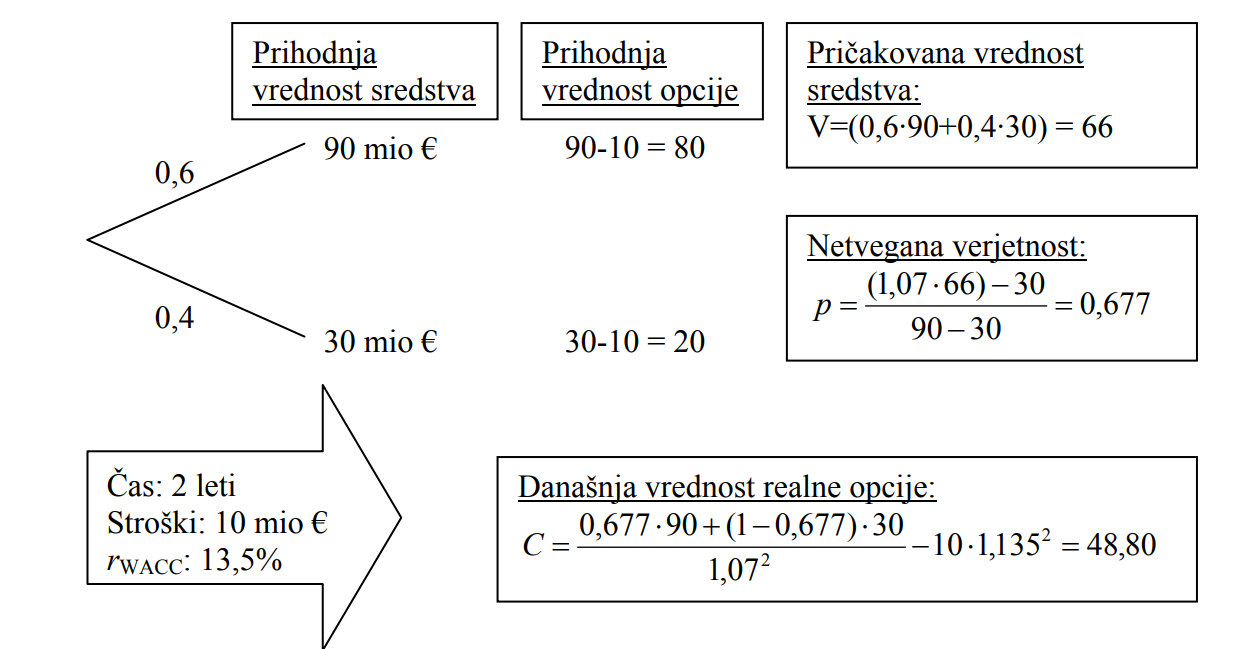
\includegraphics[width=15cm, height=9cm]{binomski_model}
(Vir: \cite[str. 24]{Mohar})

\subsection{Vrste realnih opcij in primeri uporabe}
V tem poglavju bom poskušal prikazati uporabo realnih opcij v praksi. S pomočjo odločitvenega drevesa bom poskušal prikazati osnovno uporabo in prepoznavanje tržnih razmer. Še posebej se bom osredotočil na opcije, ki omogočajo opustitev projekta, njegovo razširitev ali začasno zaustavitev. \\

Videli bomo lahko, da je uporaba tradicionalnih metod pri vrednotenju realnih sredstev napačna oziroma njena uporaba ni priporočljiva, zaradi fleksibilnosti managementa, ki lahko prilagodijo ali prestavijo odločitev. Vrednost managerske prilagodljivosti lahko bolje opišemo z razširjenim NSV pravilom \cite[str. 151, 152]{Trigeorgis}:
\begin{center}
$Razširjena\;NSV = NSV + premija\;za\;opcijo$.
\end{center}
Tradicionalne metode so bile razvite za vrednotenje obveznic in delnic, pri katerih investitorji niso upoštevali realnih sredstev podjetja. Pri uporabi tradicionalnih metod se predpostavlja, da so managerske odločitve sprejete samo na začetku. Zato bomo v primerih spodaj uporabili odločitveno drevo, ki najbolje upošteva aktivnost managementa. V odločitvenem drevesu je aktivnost predstavljena kot možnost, da se management čez čas odloči za odločitev, predvsem takrat, ko bo nekaj negotovosti že znane \cite[str. 152]{Trigeorgis}. \\

\subsubsection{Osnovna naloga}
Predpostavimo, da želimo vrednotiti investicijo (izgradnja tovarne), ki zahteva začetni vložek v višini $I_0= 104$ mio €. Investicija bo naslednje leto prinesla $180$ mio €, če bodo tržne razmere dobre ($V^+=180$), in $60$ mio €, če bodo razmere slabe ($V^-=60$). To je binomsko drevo, kjer vrednost $V$ ob času 0 pomnožimo s faktorjem $u=1,8$, če je trg ugoden in s faktorjem $d=0,6$, če ne. Verjetnost, da bodo tržne razmere dobre ali slabe, je enaka in sicer $q=0,5$ \cite[str. 153]{Trigeorgis}. \\
Da bomo lahko določili neto sedanjo vrednost, pa želimo oceniti tudi oportunitetni strošek kapitala. Če stopnja tveganja pri investiciji ni enaka povprečni stopnji tveganja vseh investicij podjetja, potem uporaba stroška kapitala podjetja ne bo ustrezna. Za izračun stopnje donosa si zamislimo vrednosti papir, ki je na las podoben naši investiciji. Naj s $S$ označimo vrednost tega papirja, s katerim se trguje na finančnih trgih in je podobno tvegan kot naša investicija. Tak vrednostni papir je ustvarjen z namenom izračuna željene stopnje donosa naše investicije. Današnja vrednost papirja je $S=20$ €, trg pa se obnaša enako kot pri naši investiciji. Tako lahko izračunamo pričakovano stopnjo donosa $k$ kot \cite[str. 153, 154]{Trigeorgis}:
\begin{center}
$k = \tfrac{E_0(S_1)}{S_0}-1= \tfrac{0,5 * (20*1,8)+0,5*(20*0,6)}{20}-1= 0,2 = 20 \%$,
\end{center}
kjer z $E_0(S_1)$ označimo pričakovano vrednost papirja. Predpostavimo tudi, da je netvegana obrestna mera enaka $8 \%$.\\

\subsubsection{Uporaba tradicionalne metode}
Po osnovni formuli lahko hitro izračunamo vrednost investicije ob času 0 \cite[str. 154]{Trigeorgis}:
\begin{center}
$V_0 = \tfrac{qV^+  + (1-q)V^-}{1+k}= \tfrac{0,5 * 180+0,5*60}{1+0,2}= 100$.
\end{center}
Tako dobimo vrednost NSV:\\
$NSV = 100 - 104 = -4$.\\
Se pravi je vrednost investicije ob času 0 enaka $-4$ mio €. Če bi sledili logiki, bi investicijo zavrnili.\\
Tradicionalne metode vrednotenja so tako povsem neuporabne pri realnih opcijah, saj ne upoštevajo prihodnjih dogodkov, ki so v času začetka investicije še negotovi. Zato so se tudi skozi čas razvile metode, ki bi pripomogle k razreševanju podobnih problemov. V nadaljevanju pa bom opisal metodo, ki pripomore pri izračunu realnih opcijah \cite[str. 154]{Trigeorgis}.\\

Kot pa bomo lahko opazili v nadaljevanju, največja napaka tradicionalnih metod leži v vrednotenju investicijske priložnosti, pri katerih zahteve niso simetrične. Nesimetričnost zahtev pa izhaja iz fleksibilnosti managementa, ki lahko spremeni celoten potek \cite[str. 155]{Trigeorgis}. \\

\subsubsection{Metoda pogojnih terjatev}
Metoda pogojnih terjatev je ena izmed zelo uporabnih metod za vrednotenje realnih opcij in omogoča izračun dodatne vrednosti, ki jo prinaša uporaba fleksibilnosti. Ob odsotnosti fleksibilnosti, pa metoda izračuna popolnoma enake zneske kot tradicionalne metode.  \\
Da opišemo metodo, predpostavimo, da se celotna vrednost investicije (v celoti dokončana investicija), označena z $V$, in vrednost identičnega vrednostnega papirja $S$ gibljeta skozi prvo obdobje enako (z istimi verjetnostnimi in faktorji). V našem primeru pa ne smemo zamešati vrednost v celoti dokončane investicije z vrednostjo, ki jo določa priložnost za začetek gradnje nove tovarne. Vrednost za lastnike kapitala, da začnejo gradnjo nove tovarne, označimo jo z $E$, se giblje povsem enako kot $V$ in $S$  \cite[str. 155, 156]{Trigeorgis}.\\
Sedaj pa lahko predpostavimo, da na trgu obstaja možnost, da oblikujemo portfelj $N$ delnic vrednostnega papirja z vrednostjo $S$, kjer to financiramo z izposojenim denarjem v višini $B$ in obrestno mero $r$. Ta portfelj lahko izberemo tako, da ravno pokrije izplačila lastniškega kapitala (oziroma investicijske priložnosti) \cite[str. 156]{Trigeorgis}. \\


\tikzstyle{bag} =  text centered]
\tikzstyle{end} = []
\begin{tikzpicture}[sloped]
  \node (a) at ( 0,0) [bag, align = left, text width=8em] {$E = NS - B$};
  \node (b) at ( 6,-2) [bag, align = right, text width=15em] {$E^- = NS^- - (1+r)B$};
  \node (c) at ( 6,2) [bag, align = right, text width=15em] {$E^+ = NS^+ - (1+r)B$};
  \draw [->] (a) to node [below] {$1-q$} (b);
  \draw [->] (a) to node [above] {$q$} (c);
\end{tikzpicture}
\\[0,5 cm]

Če je portfelj izbran skrbno, potem je vrednost investicijske priložnosti, $E$, enaka vrednosti portfelja. Iz enačb za identična izplačila dobimo vrednosti $N$ in $B$ \cite[str. 156]{Trigeorgis}:
\begin{center}
$N = \tfrac{E^+ - E^-}{S^+ - S^-}$\\[0,5 cm]
$B = \tfrac{E^+S^- - E^-S^+}{(S^+ - S^-)(1+r)} = \tfrac{NS^- - E^-}{1+r}$\\
\end{center}
Z drugimi besedami, management lahko poustvari izplačila lastniškega kapitala z nakupom $N$ delnic vrednostnega papirja, ki jih financira z izposojenim denarjem v višini $B$ z obrestno mero $r$. Ko v enačbo za $E$ vstavimo izračunani $N$ in $B$ dobimo \cite[str. 156, 157]{Trigeorgis}:
\begin{center}
$E = \tfrac{\rho E^+ + (1-\rho)E^-}{1+r}$, kjer je \\[0,5 cm]
$\rho = \tfrac{(1+r)S - S^-}{S^+ - S^-} = \tfrac{(1+r)-d}{u-d}$
\end{center}
Tako lahko opazimo, da investicijska priložnost ne vsebuje verjetnosti $q$, ampak vsebuje do tveganja nevtralno verjetnost $\rho$, ki omogoča diskontiranje pričakovanih vrednosti po nevtralni obrestni meri. \\

Preden nadaljujemo z opisom in reševanjem problema realnih opcij, pa za začetek razširimo naše binomsko drevo na 2 leti. Prva vrednost v drevesu označuje vrednost $V$, druga pa vrednost identičnega vrednostnega papirja $S$ \cite[str. 158]{Trigeorgis}. \\[0,5 cm]

\tikzstyle{bag} = [text width=5em, text centered]
\tikzstyle{end} = []
\begin{tikzpicture}[sloped]
  \node (a) at ( 0,0) [bag] {$100$; $20$};
  \node (b) at ( 4,-1.5) [bag] {60; 12};
  \node (c) at ( 4,1.5) [bag] {180; 36};
  \node (d) at ( 8,-3) [bag] {36; 7,2};
  \node (e) at ( 8,0) [bag] {108; 21,6};
  \node (f) at ( 8,3) [bag] {324; 64,88};
  \draw [->] (a) to node [below] {} (b);
  \draw [->] (a) to node [above] {} (c);
  \draw [->] (c) to node [below] {} (f);
  \draw [->] (c) to node [above] {} (e);
  \draw [->] (b) to node [below] {} (e);
  \draw [->] (b) to node [above] {} (d);
\end{tikzpicture}

\subsubsection{Opcija časa investiranja}
\cite[str. 158, 161]{Trigeorgis}\\
Predpostavimo, da ima podjetje enoletno licenco, ki omogoča zamik začetka investicije, v našem primeru izgradnje tovarne, za eno leto. Želimo ugotoviti kakšna je vrednost investicije zagotovljena s strani licence. Videli smo že, da če bi želeli investicijo izpeljati danes, bi to pomenilo, da bi bili na izgubi. Z licenco pa pridobijo eno leto, v katerem se lahko marsikatera negotovost razjasni, zato vrednost te opcije ne more biti enaka kot prej. Da izračunamo točno vrednost opcije čas investiranja \textit{(angl. option defer investment)}, v zgornjem binomskem drevesu na novo izračunamo vrednosti $E^+$ in $E^-$. 

Ker daje opcija časa investiranja pravico, ne pa obveznosti, da investicijo začnejo v naslednjem letu, bodo z investicijo počakali eno leto in z njo začeli v primeru, da bodo razmere ugodnejše. Z drugimi besedami to pomeni, da lahko to opcijo primerjamo z nakupno opcijo glede na vrednost celotne investicije $V$, z začetnim izdatkom v naslednjem letu, ki ga označimo kot $I_1$ ($I_1 = I_0*1,08 = 112,32)$.  Tako izračunamo:
 \begin{center}
$E^+ = max\{V^+ - I_1; 0\} = max\{180 - 112,32; 0\} = 67,68$,\\[0,5 cm]
$E^- = max\{V^- - I_1; 0\} = max\{60 - 112,32; 0\} = 0.$
\end{center}
Struktura izplačil je potem naslednja: \\

\tikzstyle{bag} =  text centered]
\tikzstyle{end} = []
\begin{tikzpicture}[sloped]
  \node (a) at ( 0,0) [bag, align = left, text width=8em] {$V_0=100, E_0=?$};
  \node (b) at ( 6,-2) [bag, align = right, text width=8em] {$V^-=60, E^-=0$};
  \node (c) at ( 6,2) [bag, align = right, text width=12em] {$V^+=180, E^+=67,68$};
  \draw [->] (a) to node [below] {$1-q$} (b);
  \draw [->] (a) to node [above] {$q$} (c);
\end{tikzpicture}


Sedaj pa lahko izračunamo vrednost $E_0$ kot: 
 \begin{center}
$E_0 = \tfrac{\rho E^+ + (1-\rho)E^-}{1+r} = \tfrac{0,4 * 67,68 + 0,6 * 0}{1,08} = 25,07 $
\end{center}
in tako dobimo vrednost investicijske priložnosti (ali razširjena NSV vrednost). Vidimo, da je v tem primeru vrednost pozitivna, kar pomeni, da se nam splača počakati eno leto. Vrednost opcije pa lahko izračunamo s formulo:\\[0,5 cm]
$Premija\;za\; opcijo = Razširjena\; NSV - NSV = 25,07 - (-4) = 29,07. $\\

\subsubsection{Opcija rasti}
\cite[str. 162, 163]{Trigeorgis}\\
Ko se management odloči, da bo investicijo podprl, potem do izraza pride njegova fleksibilnost. V vsakem trenutku lahko poseže v investicijo in konkretno spremeni nadaljnji potek. Takšna opcija je tudi opcija rasti \textit{(angl. option to expand)}. Manager se lahko odloči za povečanje oziroma razširitev tovarne, saj vidi, da je njihov novi produkt bolje prodajan, kot so predvidevali. Tako lahko originalno investicijsko priložnost vidimo kot začetna investicija plus nakupna opcija na prihodnjo priložnost.\\

Predpostavimo, da ima v našem primeru (če se je projekt začel v času 0) manager opcijo investirati dodatnih $80$ mio € eno leto po začetku (to označimo kot $I^'_1 = 80$ mio €), kar bi podvojilo proizvodnjo in vrednost tovarne oziroma investicije. Tako ima manager v letu 1 možnost, da ohrani enako proizvodnjo (brez dodatnih stroškov dobi $V$), ali pa jo poveča (dodatni stroški in podvojen zaslužek). Dobimo:\\

 \begin{center}
$E = max\{V; 2V - I^'_1\} = V + max\{V - I^'_1; 0\}$,
\end{center}
prav tako pa dobimo tudi:\\
\begin{center}
$E^+ = max\{V^+; 2V^+ - I^'_1\} =  max\{180; 360 - 80\} = 280$
\end{center}
in
\begin{center}
$E^- = max\{V^-; 2V^- - I^'_1\} =  max\{60; 120 - 80\} = 60$.
\end{center}

Tako vidimo, da bomo opcijo izvršili, če bodo tržne razmere ugodne, v nasprotnem primeru pa opcijo ne izvršimo. Sedaj lahko izračunamo investicijsko priložnost kot:
\begin{center}
$E_0 = \tfrac{\rho E^+ + (1-\rho)E^-}{1+r} - I_0= \tfrac{0,4 * 280 + 0,6 * 60}{1,08} - 104 = 33,04 $.
\end{center}
Vrednost opcije rasti je enaka $33,04-(-4)=37,04$ mio €.\\

\subsubsection{Opcija zožitve}
\cite[str. 163, 164]{Trigeorgis}\\
Opcija zožitve \textit{(angl. option to contract)} je opcija podobna opciji rasti, le da gre v tem primeru za zmanjšanje proizvodnje zaradi slabih tržnih razmer. \\

Predpostavimo, da bo v našem primeru začetna investicija za začetek izgradnje in zagotavljanje proizvodnje ($104$ mio €) porabljena naslednje leto. Bolj natančno, $50$ mio € bo potrebno plačati takoj ob začetku izgradnje, dodatnih $58,32$ mio € (to je prihodnja vrednost $54$ mio €) pa bo še potrebno plačati v naslednjem letu. Predpostavimo tudi, da ima management opcijo  prepoloviti proizvodnjo in vrednost investicije tako, da zmanjša začetni izdatek. To pomeni, da bo naslednje leto potreboval investirati zgolj $I^{''}_1 = 25$ mio € (in tako privarčeval $I^*_1 = 33,32$ mio €). Seveda, če bodo tržne razmere v naslednjem letu slabe, bo management uporabil to opcijo. Tako izračunamo:\\

\begin{center}
$E = max\{V - I_1; 0,5V - I^{''}_1\} = (V-I_1) + max\{0; I^*_1-0,5V\}$,
\end{center}
prav tako pa dobimo tudi:\\
\begin{center}
$E^+ = max\{180-58,32; 90-25\} = (180-58,32) + max\{0; 33,32-90\}= 121,68$
\end{center}
in
\begin{center}
$E^- = max\{60-58,32; 30-25\} = (60-58,32) +  max\{0; 33,32-30\} = 5$.
\end{center}

Sedaj pa ocenimo še investicijsko priložnost:\\
\begin{center}
$E_0 = \tfrac{0,4 * 121,68 + 0,6 * 5}{1,08} - 50 = -2,16 $
\end{center}
in tako je opcija vredna $-2,16-(-4) = 1,84$ mio €. \\

\subsubsection{Opcija opustitve projekta}
\cite[str. 166, 167]{Trigeorgis}\\
Ena izmed možnosti, ki se skozi projekt ponuja managementu, je tudi opcija opustitve projekta \textit{(angl. option to abandon for salvage value)}, kjer management bodisi proda svojo investicijo za tako imenovano zaščitno ceno bodisi zamenja za neko drugo sredstvo. Za ponazoritev primera si zamislimo kemijsko tovarno, ki lahko za svoje obratovanje uporablja elektriko ali premog in ima možnost proizvajati vitamine ali pa aspirine. Logično je, da ko se cene premoga, elektrike, vitaminov in aspirinov na trgu spreminjajo, bodo lastniki podjetje želeli prestrukturiranje, zato je pomembno, da znamo določiti vrednost opcije. Zamislimo si, da se zaščitna cena giblje kot je prikazano spodaj . \\
\\

\tikzstyle{bag} = [text width=5em, text centered]
\tikzstyle{end} = []
\begin{tikzpicture}[sloped]
  \node (a) at ( 0,0) [bag] {$85$};
  \node (b) at ( 4,-1.5) [bag] {$68$};
  \node (c) at ( 4,1.5) [bag] {$127,5$};
  \node (d) at ( 8,-3) [bag] {$54,4$};
  \node (e) at ( 8,0) [bag] {$102$};
  \node (f) at ( 8,3) [bag] {$191$};
  \draw [->] (a) to node [below] {} (b);
  \draw [->] (a) to node [above] {} (c);
  \draw [->] (c) to node [below] {} (f);
  \draw [->] (c) to node [above] {} (e);
  \draw [->] (b) to node [below] {} (e);
  \draw [->] (b) to node [above] {} (d);
\end{tikzpicture}

Trenutna zaščitna cena je manj vredna kot sedanja vrednost investicija ($V = 100$), saj bi drugače management uporabil opcijo že danes. Gibanje zaščitne cene je postavljeno tako, da v primeru, da bodo tržne razmere ugodne, se opustitev ne bo zdela optimalna odločitev, v primeru slabih razmer, pa bo opustitev zelo privlačna odločitev. Z drugimi besedami povedano, vrednost določimo kot maksimum med vrednostjo investicije in zaščitno ceno.
\begin{center}
$E^+ = max\{V^+; A^+\}= max\{180; 127,5\} = 180$ (nadaljujemo investicijo), \\[0,5 cm]
$E^- = max\{V^-; A^-\}= max\{60; 68\} = 68$ (opustimo investicijo). \\[0,5 cm]
\end{center}

Vrednost investicijske priložnosti (ta vrednost vključuje tudi vrednost, da opustimo investicijo že zgodaj ali pa jo zamenjamo po 1 letu) je tako enaka: \\[0,5 cm]
\begin{center}
$E_0 = \tfrac{\rho E^+ + (1-\rho)E^-}{1+r}-I_0 = \tfrac{0,4*180+0,6*68}{1,08} -104 = 0,44$. 
\end{center}

Vrednost opcije pa je $0,44-(-4)=4,44$ mio €. \\

S tem sem zaključil in ponazoril nekatere osnovne vrste realnih opcij in omogočil lažje razumevanje njihove uporabe v praksi.


\pagebreak
\begin{center}
\large{Slovar strokovnih izrazov}
\end{center}

\begin{table}[ht]
\centering
\setlength\extrarowheight{8pt}
\begin{tabular}{|l|l|}
\hline
\textbf{Angleško} & \textbf{Slovensko} \\
\hline
\hline
  IRR - internal rate of return      &  Notranja stopnja donosa         \\
\hline
    The income approach     &     Dohodkovni pristop      \\
\hline
    The marker approach     &    Tržni pristop      \\
\hline
      The cost approach   &     Stroškovni pristop      \\
\hline
      WACC -  weighted average cost of capital  &   Povprečni strošek kapitala        \\
\hline
  NPV - net present value  &        NSV - neto sedanja vrednost   \\
\hline
     Payback period    &      Doba povračila     \\
\hline
    Call option     &       Nakupna opcija    \\
\hline
    Put option     &      Prodajna opcija     \\
\hline
     Option holder    &       Dolga stran    \\
\hline
     Option writer    &       Kratka stran \\   
\hline
	Option premium & Premija za opcijo \\
\hline
	At-the-money & Opcija na meji \\
\hline
	In-the-money & Opcija se splača \\
\hline
	Out-of-the-money & Opcija se ne splača\\
\hline
	Equity options & Kapitalske opcije \\
\hline
	Option to defer investment & Opcija časa investiranja \\
\hline
	Option to expand & Opcija rasti \\
\hline
	Option to contract & Opcija zožitve \\
\hline
	Option to abandon & Opcija opustitve \\
\hline	
\end{tabular}
\end{table}


\pagebreak
\begin{thebibliography}{99}

\bibitem{Brach}
M.A.~Brach, \emph{Real options in practice}, John Wiley \& Sons, Inc., New Jersey, 2003.

\bibitem{investopedia}
J.~Chen, \emph{Risk}, [ogled 5.~5.~2021], dostopno na \url{https://www.investopedia.com/terms/r/risk.asp}.

\bibitem{Crnigoj}
M.~Črnigoj, \emph{Poslovne finance 1}, prosojnice predavanja pri predmetu Poslovne finance 1, Ekonomska fakulteta, Univerza v Ljubljani, 2021.

\bibitem{Groppelli}
A.A.~Groppelli in E.~Nikbakht, \emph{Finance}, \textbf{4}, Barron's Educational Series, Hauppauge (N.Y.), 2000.

\bibitem{Keown}
A.J.~Keown, J.D.~Martin, J.W.~Petty in D.F.~Scott, \emph{Financial management: principles and applications}, \textbf{10}, Pearson/Prentice Hall, Upper Saddle River (N.J.), 2005.

\bibitem{Kosir}
T.~Košir, K.~Pugelj, A.~Toman, \emph{Dodatno gradivo za pripravo na tekmovanje v znanju finančne matematike in statistike}, verzija 2016, [ogled 10.~5~2021], dostopno na \url{http://www.dmfa.si/Tekmovanja/Gradiva/FMS_gradivo_2016.pdf}.

\bibitem{Lenarcic}
M.~Lenarčič, \emph{Vrednotenje naložbe: realne opcije pri investicijskem odločanju}, specialistično delo, Ekonomska fakulteta, Univerza v Ljubljani, 2002.

\bibitem{Mohar}
E.~Mohar, \emph{Uporaba realnih opcij v praksi}, diplomsko delo, Ekonomska fakulteta, Univerza v Ljubljani, 2005.

\bibitem{Mramor}
D.~Mramor, \emph{Osnove poslovnih financ 2}, Ekonomska fakulteta , Ljubljana, 1993.

\bibitem{Mun}
J.~Mun, \emph{Real options analysis}, \textbf{2}, John Wiley \& Sons, Inc., 2006.

\bibitem{Trigeorgis}
L.~Trigeorgis, \emph{Real options}, Managerial flexibility and strategy in resource allocation, The MIT Press Cambridge, Massachusetts (London), 2000.







\end{thebibliography}
\end{document}
